%卒論概要テンプレート ver. 4.0

\documentclass[uplatex,twocolumn,dvipdfmx]{jsarticle}
\usepackage[top=22mm,bottom=22mm,left=22mm,right=22mm]{geometry}
\setlength{\columnsep}{11mm}
\usepackage[T1]{fontenc}
\usepackage{txfonts}
\usepackage[expert,deluxe]{otf}
\usepackage[dvipdfmx,hiresbb]{graphicx}
\usepackage[dvipdfmx]{hyperref}
\usepackage{pxjahyper}
\usepackage{secdot}





%タイトルと学生番号,名前だけ編集すること
\title{\vspace{-5mm}\fontsize{14pt}{0pt}\selectfont Twitterにおけるデマ拡散のシミュレーション}
\author{\normalsize プロジェクトマネジメントコース 矢吹研究室 1442043 川崎貴雅}
\date{}
\pagestyle{empty}
\begin{document}
\fontsize{10.5pt}{\baselineskip}\selectfont
\maketitle



%以下が本文
\section{序論}\label{序論}

Twitterはリアルタイムな情報を手軽に多くのユーザーへと伝播できるため社会に影響を与えている.\#MeTooというハッシュタグの投稿により性的被害やセクハラについて考えるきっかけが,世界中に広がった事が挙げられる.
しかし悪い影響を与えてしまう場合もある.例えば東日本大震災時のデマ情報が拡散された事や北朝鮮のミサイルを目撃したというデマが挙げられる.このようなツイートの拡散をシミュレーションで再現することを試みる.
本研究ではTwitterでのデマの拡散をシミュレーションで再現することができるかを調査したい.
実際にデマ拡散シミュレーションを行うために,人は1日にどのくらいツイートする数の確認とツイートが拡散する様子をシュミレートする手法の確立を行う.

\section{目的}

本研究では現実のデマ拡散に近い状況を再現できるシミュレーションの開発である.

\section{手法}

以下の手順でデマの拡散をシミュレートする.
\begin{enumerate}
\item TwitterAPIを用いて50万人のユーザーから1日のユーザー数に1日のツイート数とフォロー数,フォロワー数の取得を行い,それをもとに1日あたりのツイート数の分布を出す.
\item ツイートの拡散する様子をシュミレートする手法を確立するために,1から10までが0.2の確率でつながってるランダムグラフでRTで拡散する確率が0.5のシミュレーションを試みる\cite{netto}.
\item 上記2つを組み合わせたシミュレーションを行う.
\end{enumerate}

\section{結果}

50万人のデータから1日あたりのツイート数の分布が分かった.またグループ構築にランダムグラフを使ったツイート拡散のシュミレート手法も確立できた.図\ref{何人がRTを見るか}のようにフォロー数とRTをするかの数値を動かして可視化を行えるようになった.しかし1日あたりのツイート数の分布とツイート拡散のシミュレート手法を組み合わせた現実的なシミュレーションを行うことはできなかった.

\begin{figure}[htb]
\centering
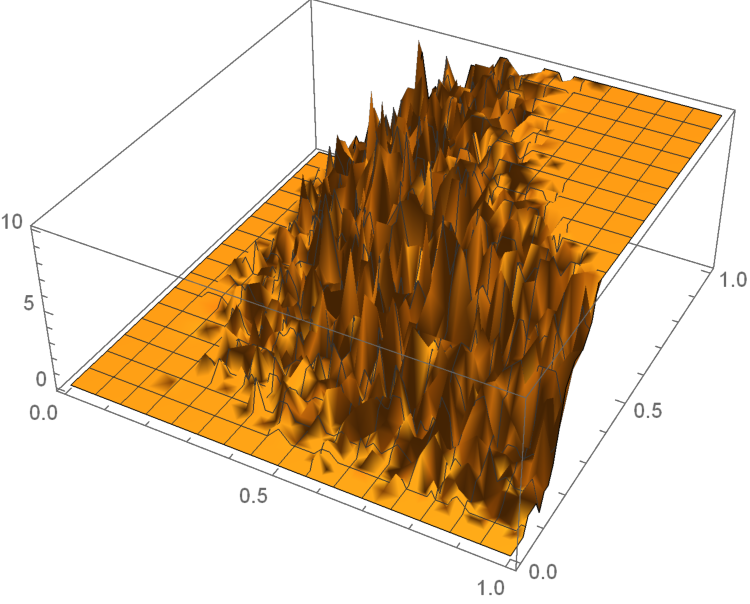
\includegraphics[width=44mm,clip]{result.pdf}
\caption{シミュレーションの可視化}\label{何人がRTを見るか}
\end{figure}

\section{考察}

10人でのシミュレーション内のメンバー全てがRTされたツイートを確認できるようになるのは互いに繋がってる確率が0.5でRTする確率が0.6を超えたあたりである.またメンバーが増えるとRTを全てのメンバーがみた時のそれぞれ確立が下がったため,メンバ増加により確立は下がると考えられる.

\section{結論}

本研究では,50万人のデータから作った1日あたりのツイート数の分布とツイート拡散のシュミレートをする手法の確立を行った.その結果1日のあたりのツイート数の分布確認,ツイートの拡散シュミレートの手法の確立が行えた.この結果を用いてシミュレーションを行うことでより現実的な物になることが期待出来る.

\bibliographystyle{junsrt}
\bibliography{biblio}%「biblio.bib」というファイルが必要.

\end{document}
